% paper.tex -- draft, A&A LaTeX class (aa.cls v7.0, EDP Sciences)
% Structure only: Equation of State, Field Equations, Castro, Braithwaite method.
% TODO: title, author list, affiliations, abstract, results/discussion sections.

\documentclass{aa}

\usepackage{graphicx}
\usepackage{amsmath}
\usepackage{amssymb}
\usepackage{txfonts}
\usepackage{natbib}

\begin{document}

   \title{Magnetized white dwarfs with mixed poloidal-toroidal fields}

   \subtitle{Draft -- a certified $2\,M_\odot$ configuration}

   \author{TBD\inst{1}
          }

   \institute{Affiliation TBD\\
              \email{tbd@example.org}
             }

   \date{Draft \today}

   \abstract
   % context
   {A white dwarf well above the Chandrasekhar mass requires support
    beyond electron degeneracy. A strong internal magnetic field can
    supply it, but a purely toroidal field has no exterior structure and
    so no dipole for magnetic braking to act on.}
   % aims
   {We construct a $2\,M_\odot$ configuration carrying both components,
    and ask what a poloidal component costs when it is added to a
    toroidal-dominated equilibrium.}
   % methods
   {The toroidal field is solved self-consistently with the stellar
    structure by a self-consistent field iteration under a cold
    degenerate equation of state. A single solve carrying both components
    is not available in barotropy, where the toroidal field is confined to
    the closed-poloidal-line region and the reachable ratio is a few
    percent, so the poloidal component is solved on the converged density
    and imposed. Every configuration is gated on the virial error, on the
    star fitting inside its domain, and on the central density staying
    below the inverse-beta-decay threshold.}
   % results
   {The configuration reaches $M = 2.007\,M_\odot$ at
    $\rho_c = 10^9$\,g\,cm$^{-3}$ with $E_{\mathrm{tor}}/|W| = 0.203$,
    a virial error of $9.9\times10^{-5}$, and a mass converging
    monotonically under mesh refinement. The field is strongly
    toroidal-dominated, $B_{\mathrm{t}}/B_{\mathrm{p}} = 884$ in energy,
    with a peak of $4.28\times10^{13}$\,G and an exterior dipole of
    $5.9\times10^{10}$\,G. The virial error of the pair tracks the
    imposed poloidal energy almost one for one, so a more balanced field
    leaves the certified regime: at
    $B_{\mathrm{t}}/B_{\mathrm{p}} = 8.8$ the virial error is twenty
    times the acceptance threshold.}
   % conclusions
   {A $2\,M_\odot$ white dwarf with a strong toroidal field and an
    exterior dipole is constructible and certifiable, at the cost of a
    poloidal component carrying a tenth of a percent of the magnetic
    energy. It is not shown to be stable: a field this toroidal is the
    configuration most exposed to the Tayler instability, which an
    axisymmetric calculation cannot test.}

   \keywords{white dwarfs -- stars: magnetic field -- magnetohydrodynamics (MHD) -- methods: numerical}

   \maketitle

%-------------------------------------------------------------------

\section{Introduction}

TBD.

%-------------------------------------------------------------------

\section{Equation of state}
\label{sec:eos}

The background stellar structure throughout this work is that of a
fully degenerate, zero-temperature electron gas
\citep[ztwd;][]{chandrasekhar1935}. Pressure and density are both
parametrized by the normalized Fermi momentum $x \equiv p_F/(m_e c)$,

\begin{align}
P(x) &= A \left[ x(2x^2-3)\sqrt{x^2+1} + 3\sinh^{-1}x \right],
\label{eq:pressure} \\
\rho(x) &= B\,x^3,
\label{eq:density}
\end{align}

\noindent where $A$ is a fixed combination of fundamental constants
($m_e$, $c$, $\hbar$) and $B$ depends on the composition only through
the mean molecular weight per electron $\mu_e = 1/Y_e$, with $Y_e$ the
number of electrons per baryon. This is a purely mechanical equation of
state: at fixed composition, pressure depends on density alone, with no
temperature dependence. Consequently, once the configuration is
restricted to be non-rotating and field-free, the entire stellar
structure (mass, radius, density profile) is determined by exactly two
physical parameters: the central density $\rho_c$ and $\mu_e$.

The specific enthalpy has a closed form,
\begin{equation}
H(x) = \frac{8A}{B}\left[\sqrt{1+x^2} - 1\right],
\end{equation}
which is what makes the self-consistent field (SCF) iteration of
Sect.~\ref{sec:field-eq} tractable: at each iteration the density is
recovered directly from the local enthalpy via the inverse relation
$x(H) = \sqrt{(1+HB/8A)^2 - 1}$, with $H \le 0$ mapped to $\rho = 0$
(the stellar surface).

Near the surface ($x \ll 1$) the equation of state reduces to
$\rho \propto H^{3/2}$, an effective polytropic index $n=3/2$; in the
relativistic core ($x \gg 1$) it approaches $\rho \propto H^3$,
$n=3$ -- the marginal polytropic index at which the equilibrium mass
becomes independent of central density, the origin of the
Chandrasekhar mass limit.

Figure~\ref{fig:eos} plots Eqs.~\ref{eq:pressure} and~\ref{eq:density}
and shows where those limits actually apply. The transition is slow: the
adiabatic index $\Gamma = \mathrm{d}\ln P/\mathrm{d}\ln\rho$ takes about
four decades in density to fall from $5/3$ to $4/3$, and neither limit is
a good description through most of that range. It also places the
configuration of Sect.~\ref{sec:results}. At its central density,
$\rho_c = 10^9$\,g\,cm$^{-3}$, the normalized Fermi momentum is
$x = 8.0$ and $\Gamma = 1.343$ -- within $0.7\%$ of the relativistic
limit. The core therefore sits essentially at the marginal index, which
matters twice over here: at $n \simeq 3$ the equilibrium is only weakly
sensitive to $\rho_c$ and correspondingly delicate, and it is also the
regime in which magnetic support translates most directly into mass,
since the magnetic energy scales with radius the same way the
gravitational and internal energies do.

\begin{figure}
\centering

\includegraphics[width=\columnwidth]{figures/eos.pdf}
\caption{The equation of state of Eqs.~\ref{eq:pressure}
and~\ref{eq:density} for $\mu_e = 2$. Upper panel: $P(\rho)$ with the two
polytropic limits, each normalized on the curve in the regime where it
holds. Lower panel: the adiabatic index, which crosses from $5/3$ to
$4/3$ over roughly four decades in density. The dashed vertical line marks the
central density of the configuration of Sect.~\ref{sec:results}, and the
point its adiabatic index there. The shaded region lies above the
inverse-beta-decay threshold for $\mu_e = 2$, where this equation of
state no longer describes a white dwarf.}
\label{fig:eos}
\end{figure}

At sufficiently high density, inverse beta decay (electron capture)
changes the composition locally and the constant-$\mu_e$ cold equation
of state above ceases to describe a real white dwarf. We adopt the
tabulated threshold densities of \citet{boshkayev2013} for this
validity limit; all central densities discussed below are kept below
this threshold for the assumed composition.

%-------------------------------------------------------------------

\section{Field equations}
\label{sec:field-eq}

\subsection{The toroidal branch}

For a barotropic star the magnetic force must derive from a potential if
hydrostatic balance is to close as a Bernoulli integral. For an
axisymmetric, purely azimuthal field
$\mathbf{B}_{\mathrm{t}} = B_\varphi\,\hat{\mathbf{e}}_\varphi$ this
restricts $B_\varphi$ to
\begin{equation}
B_\varphi = K \rho^m \varpi^{2m-1}, \qquad m \ge 1,
\label{eq:fieldlaw}
\end{equation}
with $\varpi$ the cylindrical radius, $K$ the amplitude and $m$ the
concentration towards the dense interior. The Lorentz force then follows
from a potential, $\mathbf{f}_L/\rho = -\nabla M_{\mathrm{tor}}$ with
\begin{equation}
M_{\mathrm{tor}}(s) = \frac{m K^2}{4\pi(2m-1)}\, s^{\,2m-1},
\qquad s \equiv \rho\varpi^2 ,
\label{eq:mtor}
\end{equation}
which we verified symbolically for $m = 1, 3/2, 2, 3$. Hydrostatic
equilibrium reduces to
\begin{equation}
H + \Phi + M_{\mathrm{tor}}(\rho\varpi^2) = C ,
\label{eq:bernoulli}
\end{equation}
solved together with the Poisson equation for $\Phi$ and the equation of
state of Sect.~\ref{sec:eos} by the self-consistent field iteration of
\citet{hachisu1986}. Because $M_{\mathrm{tor}}$ depends on $\rho$, the
density update is no longer a direct inversion of the equation of state
but a per-point root find; the left-hand side is monotonic in $\rho$, so
the root is unique and safely bracketed.

\subsection{The poloidal component, and why it is imposed}
\label{sec:poloidal}

An axisymmetric poloidal field derives from a flux function
$u(\varpi,z) = \varpi A_\varphi$,
\begin{equation}
B_\varpi = -\frac{1}{\varpi}\frac{\partial u}{\partial z}, \qquad
B_z = \frac{1}{\varpi}\frac{\partial u}{\partial \varpi},
\label{eq:poloidal}
\end{equation}
with $u$ obeying the Grad-Shafranov equation
\citep{grad1958,shafranov1966} sourced by the current distribution, which
we take linear in the flux.

A single self-consistent solve carrying both components is not available
in this formulation, and the obstruction is not a numerical one. In
barotropy the toroidal function must depend on the flux alone,
$\beta = \beta(u)$; since there is no current outside the star,
$B_\varphi$ must vanish on every flux surface that reaches the surface,
so the toroidal field is confined to the region of closed poloidal lines.
The energy ratio reachable that way is a few percent, far from the
toroidal-dominated configuration required below. We therefore solve the
toroidal branch self-consistently for the structure, and impose the
poloidal field on the converged density.

That imposition has a price, and Sect.~\ref{sec:tradeoff} measures it:
the imposed field's energy is precisely the term left unbalanced in the
virial, so imposing a poloidal component carrying a fraction $x$ of the
binding energy costs a virial error of about $x$. The poloidal component
adopted here is small enough that this cost stays below the acceptance
threshold, which is what makes the configuration certifiable at all.

Purely toroidal and purely poloidal equilibria are each subject to a
non-axisymmetric instability of azimuthal wavenumber $m=1$
\citep{tayler1973,markey1973}, which an axisymmetric formulation cannot
test for. Sect.~\ref{sec:limitations} returns to this.

%-------------------------------------------------------------------

\section{Results}
\label{sec:results}

\subsection{A certified $2\,M_\odot$ configuration}
\label{sec:certified}

Table~\ref{tab:config} reports the configuration this paper is about: a
non-rotating white dwarf of $2.007\,M_\odot$ at
$\rho_c = 10^9$\,g\,cm$^{-3}$, carrying a toroidal field with
$E_{\mathrm{tor}}/|W| = 0.2026$ and a poloidal component imposed on top.

\begin{table}
\caption{The adopted configuration. $\mu_e = 2$, $m = 1$, no rotation.}
\label{tab:config}
\centering
\begin{tabular}{l r}
\hline\hline
$\rho_c$ (g\,cm$^{-3}$)                        & $1.0\times10^{9}$ \\
$M$ ($M_\odot$)                                & 2.007 \\
$K$                                            & $3.245\times10^{-3}$ \\
$E_{\mathrm{tor}}/|W|$                         & 0.2026 \\
$B_{\varphi,\max}$ (G)                         & $4.275\times10^{13}$ \\
$B_{\mathrm{pole}}$ (G)                        & $5.91\times10^{10}$ \\
$B_{\mathrm{t}}/B_{\mathrm{p}}$ (energy)       & 884 \\
$B_{\mathrm{t}}/B_{\mathrm{p}}$ (amplitude)    & 26.2 \\
$E_{\mathrm{pol}}/E_{\mathrm{mag}}$            & $1.1\times10^{-3}$ \\
VE                                             & $9.9\times10^{-5}$ \\
$f_{\mathrm{pol}}$                             & 0.142 \\
\hline
\end{tabular}
\end{table}

The mass gain is the whole point of the toroidal field: the same central
density and composition without a field give $1.346\,M_\odot$, so the
field is carrying $+49\%$. That gain is available at a central density
well below the inverse-beta-decay threshold for $\mu_e = 2$
($1.94\times10^{10}$\,g\,cm$^{-3}$, Sect.~\ref{sec:eos}), so the
configuration is a white dwarf in the sense the equation of state can
still describe.

The field is toroidal-dominated by a wide margin,
$B_{\mathrm{t}}/B_{\mathrm{p}} = 884$ in energy and $26$ in amplitude.
The two differ because energy goes as the square and the components
occupy different volumes: the toroidal field is confined to the interior
while the poloidal one extends through the star and beyond it. Calling
this a mixed field is accurate but should not be read as balanced -- the
poloidal component carries a tenth of a percent of the magnetic energy.
What it does carry is the exterior structure, which the toroidal
component cannot have at all: $B_\varphi$ vanishes with the density, so a
purely toroidal star has no field outside it and no dipole for magnetic
braking to act on. The poloidal component supplies a surface dipole of
$5.9\times10^{10}$\,G.

One number worth stating next to the field strength. The critical field
at which Landau quantization changes the electron equation of state is
$B_c = m_e^2c^3/e\hbar = 4.414\times10^{13}$\,G, and the peak field here
is $0.97\,B_c$ -- just below it. The equation of state used has no field
dependence, so a configuration above $B_c$ would be inconsistent with its
own microphysics; this one sits at the edge of that regime rather than
inside it.

\subsection{Convergence}
\label{sec:convergence}

Figure~\ref{fig:convergence} shows the configuration under mesh
refinement at fixed domain, halving $\Delta r$ four times. The mass
converges monotonically with shrinking increments -- $0.15\%$, $0.04\%$,
$0.01\%$ -- to $2.007\,M_\odot$, and $E_{\mathrm{tor}}/|W|$ is converged
to four significant figures at every resolution beyond the coarsest.

The virial error stays below the $10^{-3}$ acceptance threshold at all
four resolutions, but it is not monotonic: it dips at the second
resolution and settles near $10^{-4}$. We report this rather than
smoothing it over, because it means the virial error at a single
resolution is not an error estimate for this configuration; the mass
convergence is. The same non-monotonicity appears at larger $K$ in this
branch, where it does cross the threshold; here it does not.

The domain was sized by the criterion that the star's polar radius clear
the boundary, $f_{\mathrm{pol}} = 0.142$ against the $0.2$ limit adopted
for this branch, and the configuration is reached by continuation in $K$
from the field-free solution, since direct solves at this amplitude do
not converge.

\begin{figure}
\centering
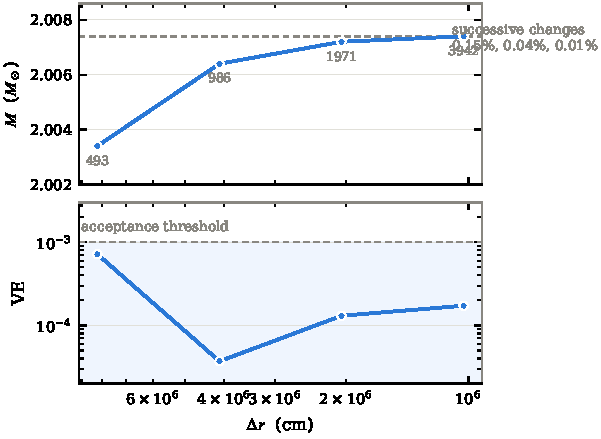
\includegraphics[width=\columnwidth]{figures/convergence_2msun.pdf}
\caption{Mesh convergence of the adopted configuration at fixed domain,
labelled by radial resolution. Upper panel: the mass, converging
monotonically to $2.007\,M_\odot$; the dashed line is the finest value.
Lower panel: the virial error, which stays inside the acceptance band
(shaded) at every resolution without being monotonic.}
\label{fig:convergence}
\end{figure}

\subsection{What the poloidal component costs}
\label{sec:tradeoff}

The poloidal field is imposed rather than solved for, so it leaves the
pair out of virial balance by its own energy. Figure~\ref{fig:tradeoff}
measures that directly: as the poloidal amplitude is raised, the virial
error of the combined configuration tracks $E_{\mathrm{pol}}/|W|$ almost
one for one, and the pair leaves the certified band once the exterior
dipole exceeds roughly $10^{11}$\,G.

This sets the configuration adopted above. At
$B_{\mathrm{t}}/B_{\mathrm{p}} = 884$ the virial error is
$9.9\times10^{-5}$, an order of magnitude inside the threshold, and the
exterior dipole is $5.9\times10^{10}$\,G. Reaching a more balanced field
is possible but not certifiable by the standard applied here: at
$B_{\mathrm{t}}/B_{\mathrm{p}} = 8.8$ the virial error is
$2.3\times10^{-2}$, twenty times the threshold. A configuration in that
range would have to be justified dynamically -- loaded into an
evolutionary calculation and allowed to relax -- rather than presented as
an equilibrium.

\begin{figure}
\centering
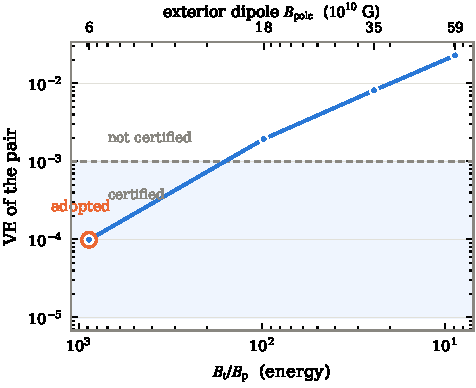
\includegraphics[width=\columnwidth]{figures/tradeoff_2msun.pdf}
\caption{The cost of the poloidal component. Moving left to right, the
imposed poloidal amplitude rises, the field becomes less
toroidal-dominated, and the exterior dipole (upper axis) grows; the
virial error of the pair rises with it and leaves the certified band
(shaded). The circled point is the configuration of
Table~\ref{tab:config}.}
\label{fig:tradeoff}
\end{figure}

%-------------------------------------------------------------------

\section{Limitations}
\label{sec:limitations}

\paragraph{No stability test.} This is a two-dimensional axisymmetric
equilibrium, certified to satisfy hydrostatic and virial balance and
nothing more. A field this strongly toroidal is precisely the
configuration subject to the Tayler $m=1$ instability
\citep{tayler1973,markey1973}, which is non-axisymmetric and therefore
invisible to this formulation by construction. The poloidal component
adopted here is far too weak to be the stabilizing agent that a mixed
field is supposed to provide. Whether this configuration survives a
non-axisymmetric perturbation is open, and answering it requires a
three-dimensional magnetohydrodynamic evolution.

\paragraph{The poloidal component is not self-consistent.} It is solved
on the converged toroidal density and imposed, for the reason given in
Sect.~\ref{sec:poloidal}: barotropy does not deliver a strongly mixed
equilibrium. The resulting virial error is small enough to certify, but
the configuration is not a solution of a single set of equations carrying
both components.

\paragraph{The equation of state does not respond to the field.} At
$0.97\,B_c$ the peak field is at the edge of the regime where Landau
quantization modifies the degenerate electron gas, and the
inverse-beta-decay threshold used to bound $\rho_c$ would itself shift
with field \citep{das2014}. Neither effect is included. Staying below
$B_c$ keeps the configuration self-consistent in this respect, but only
barely, and it forecloses raising $K$ further at this central density.

\paragraph{Barotropy.} The star is described by a cold, temperature-independent
equation of state, so it has no entropy stratification and no buoyancy
restoring force. Stable magnetic equilibria in stars are usually argued
to rely on stable stratification, which this model does not have; whether
that is a limitation of the model or a statement about degenerate stars
is beyond what these calculations can settle.

\begin{acknowledgements}
TBD.
\end{acknowledgements}

%-------------------------------------------------------------------

\bibliographystyle{aa}
\bibliography{paper}

\end{document}
